\documentclass[a4paper,12pt]{extarticle}
\usepackage[utf8x]{inputenc}
\usepackage[T1,T2A]{fontenc}
\usepackage[russian]{babel}
\usepackage{hyperref}
\usepackage{indentfirst}
\usepackage{listings}
\usepackage{color}
\usepackage{here}
\usepackage{array}
\usepackage{multirow}
\usepackage{graphicx}

\usepackage{amsmath}

\usepackage{caption}
\renewcommand{\lstlistingname}{Программа} % заголовок листингов кода

\bibliographystyle{ugost2008ls}

\usepackage{listings}
\lstset{ %
extendedchars=\true,
keepspaces=true,
language=C,						% choose the language of the code
basicstyle=\footnotesize,		% the size of the fonts that are used for the code
numbers=left,					% where to put the line-numbers
numberstyle=\footnotesize,		% the size of the fonts that are used for the line-numbers
stepnumber=1,					% the step between two line-numbers. If it is 1 each line will be numbered
numbersep=5pt,					% how far the line-numbers are from the code
backgroundcolor=\color{white},	% choose the background color. You must add \usepackage{color}
showspaces=false				% show spaces adding particular underscores
showstringspaces=false,			% underline spaces within strings
showtabs=false,					% show tabs within strings adding particular underscores
frame=single,           		% adds a frame around the code
tabsize=2,						% sets default tabsize to 2 spaces
captionpos=t,					% sets the caption-position to top
breaklines=true,				% sets automatic line breaking
breakatwhitespace=false,		% sets if automatic breaks should only happen at whitespace
escapeinside={\%*}{*)},			% if you want to add a comment within your code
postbreak=\raisebox{0ex}[0ex][0ex]{\ensuremath{\color{red}\hookrightarrow\space}},
texcl=true,
inputpath=listings,                     % директория с листингами
}

\usepackage[left=2cm,right=2cm,
top=2cm,bottom=2cm,bindingoffset=0cm]{geometry}

%% Нумерация картинок по секциям
\usepackage{chngcntr}
\counterwithin{figure}{section}
\counterwithin{table}{section}

%%Точки нумерации заголовков
\usepackage{titlesec}
\titlelabel{\thetitle.\quad}
\usepackage[dotinlabels]{titletoc}

%% Оформления подписи рисунка
\addto\captionsrussian{\renewcommand{\figurename}{Рисунок}}
\captionsetup[figure]{labelsep = period}

%% Подпись таблицы
\DeclareCaptionFormat{hfillstart}{\hfill#1#2#3\par}
\captionsetup[table]{format=hfillstart,labelsep=newline,justification=centering,skip=-10pt,textfont=bf}

%% Путь к каталогу с рисунками
\graphicspath{{fig/}}


\begin{document}	% начало документа

% Титульная страница
\begin{titlepage}	% начало титульной страницы

	\begin{center}		% выравнивание по центру

		\large Санкт-Петербургский Политехнический Университет Петра Великого\\
		\large Институт компьютерных наук и технологий \\
		\large Кафедра компьютерных систем и программных технологий\\[6cm]
		% название института, затем отступ 6см
		
		\huge Телекоммуникационные технологии\\[0.5cm] % название работы, затем отступ 0,5см
		\large Отчет по лабораторной работе №4\\[0.1cm]
		\large Аналоговая модуляция\\[5cm]

	\end{center}


	\begin{flushright} % выравнивание по правому краю
		\begin{minipage}{0.25\textwidth} % врезка в половину ширины текста
			\begin{flushleft} % выровнять её содержимое по левому краю

				\large\textbf{Работу выполнил:}\\
				\large Соболь В.О.\\
				\large {Группа:} 33501/4\\
				
				\large \textbf{Преподаватель:}\\
				\large Богач Н.В.

			\end{flushleft}
		\end{minipage}
	\end{flushright}
	
	\vfill % заполнить всё доступное ниже пространство

	\begin{center}
	\large Санкт-Петербург\\
	\large \the\year % вывести дату
	\end{center} % закончить выравнивание по центру

\thispagestyle{empty} % не нумеровать страницу
\end{titlepage} % конец титульной страницы

\vfill % заполнить всё доступное ниже пространство

% Содержание
% Содержание
\renewcommand\contentsname{\centerline{Содержание}}
\tableofcontents
\newpage




\section{Цель работы}

Познакомиться со средствами генерации и визуализации сигналов.
\section{Программа работы}

В коммандном окне MATLAB и в среде Simulink промоделировать сигналы из Главы 3, сс. 150-170 
(А.Б. Сергиенко Цифровая обработка сигналов).
\section{Теоретическая информация}

Основной задачей цифровой обработки сигналов является переход от 
аналогового сигнала, который является непрерывной функцией времени, к
дискретному сигналу. Для этого задаются частотой дискретизации, на её основе 
формируют временной ряд и считают значения сигнала в дискретные моменты времени (отсчёты).

При анализе сигналов часто используют спектр сигнала. Для получения спектра сигнал,
который является функцией времени, переводят в функцию частоты. Для этого используется преобразование Фурье.
\section{Ход выполнения работы}

\subsection{Визуализация дискретного сигнала}
\begin{figure}[H]
	\begin{center}
		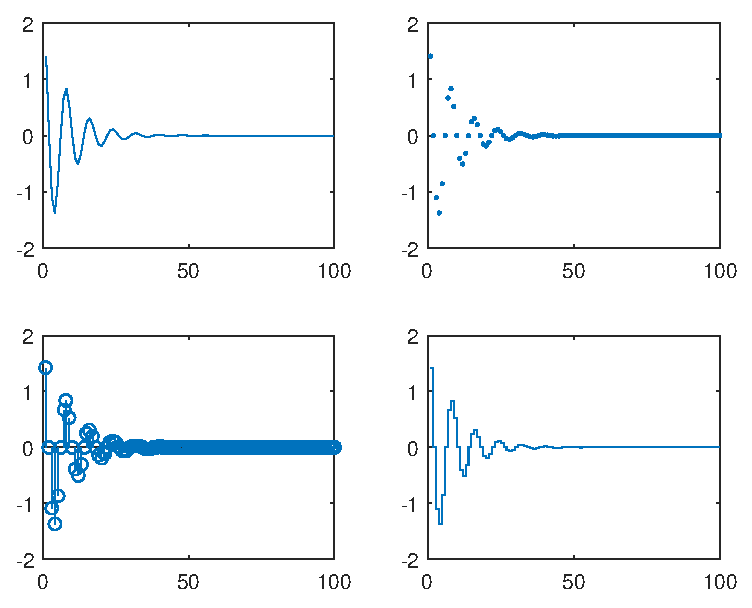
\includegraphics[scale=0.7]{lab1_01}
		\caption{Различные виды представления дискретного сигнала} 
		\label{pic:lab1_01} % название для ссылок внутри кода
	\end{center}
\end{figure}

\begin{figure}[H]
	\begin{center}
		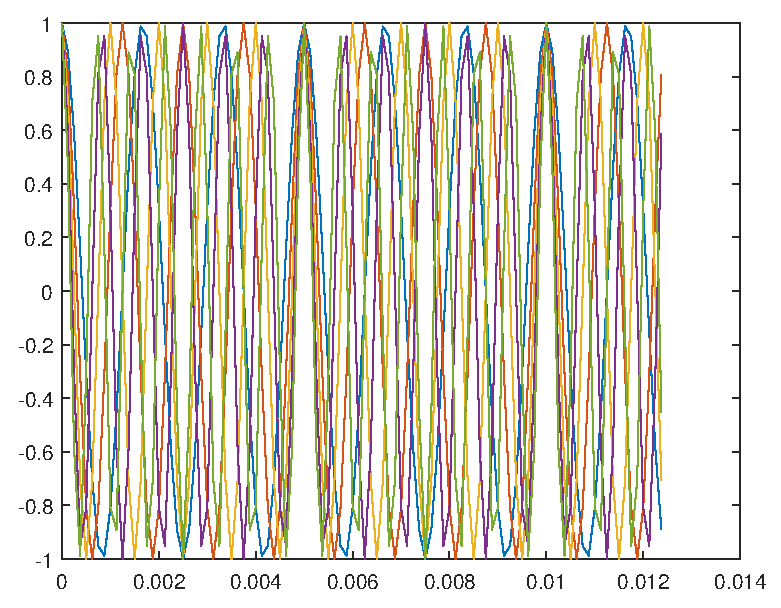
\includegraphics[scale=0.7]{lab1_03}
		\caption{Многоканальный сигнал} 
		\label{pic:lab1_03} % название для ссылок внутри кода
	\end{center}
\end{figure}

\subsection{Генерация кусочных зависимостей}
Моделирование отсчётов сигнала, который описывается разными функциями для разных 
промежутков времени.

\begin{figure}[H]
	\begin{center}
		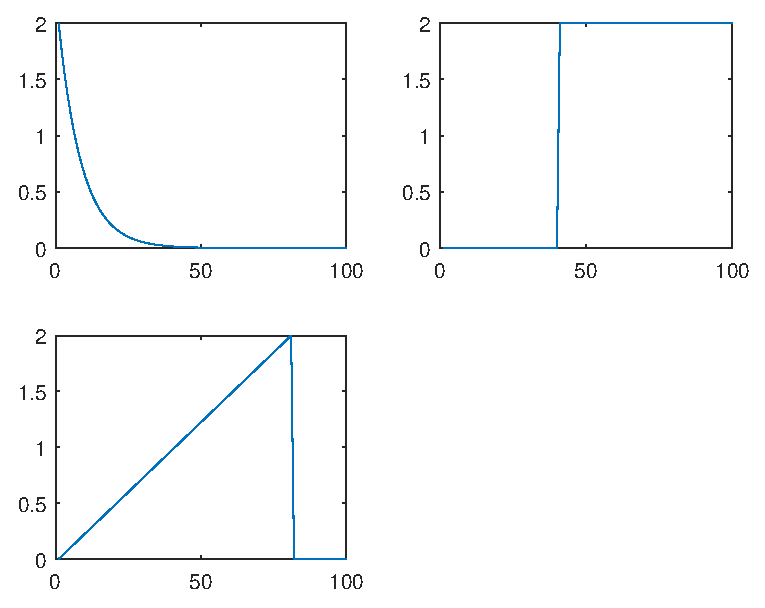
\includegraphics[scale=0.7]{lab1_04}
		\caption{Одиночные импульсы} 
		\label{pic:lab1_04} % название для ссылок внутри кода
	\end{center}
\end{figure}


\subsubsection{Прямоугольный импульс}
\begin{eqnarray}
y =
\begin{cases}
1, & \text{если } -\frac{width}{2} \leq t < \frac{width}{2}\\
0, & \text{если } t<-\frac{width}{2} , t \geq \frac{width}{2}
\end{cases}
\end{eqnarray}

\begin{figure}[H]
	\begin{center}
		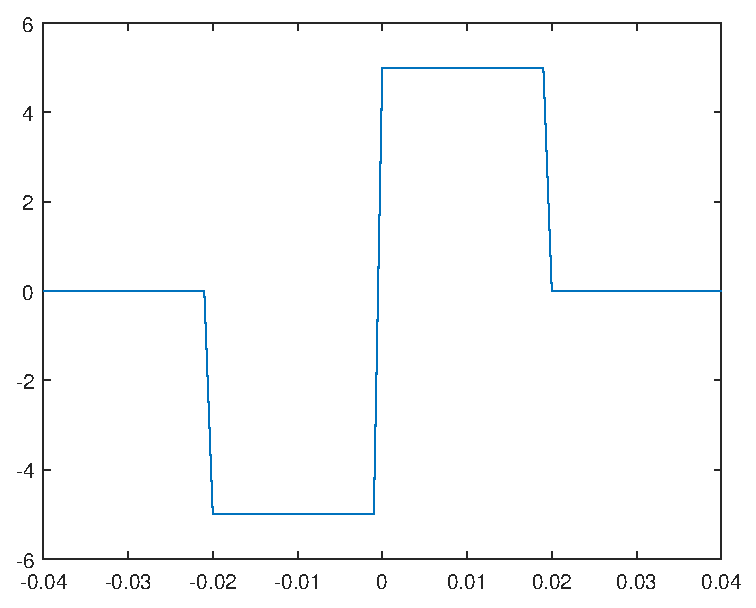
\includegraphics[scale=0.7]{lab1_05}
		\caption{Прямоугольный импульс} 
		\label{pic:lab1_05} % название для ссылок внутри кода
	\end{center}
\end{figure}
\subsubsection{Треугольный импульс}
\begin{eqnarray}
y =
\begin{cases}
\frac{2t+width}{width(skew+1)}, & -\frac{width}{2}\leq t < \frac{width*skew}{2}\\
\frac{2t-width}{width(skew-1)}, &  \frac{width*skew}{2}\leq t < \frac{width}{2}\\
0, & |t| > \frac{width}{2}
\end{cases}
\end{eqnarray}
\begin{figure}[H]
	\begin{center}
		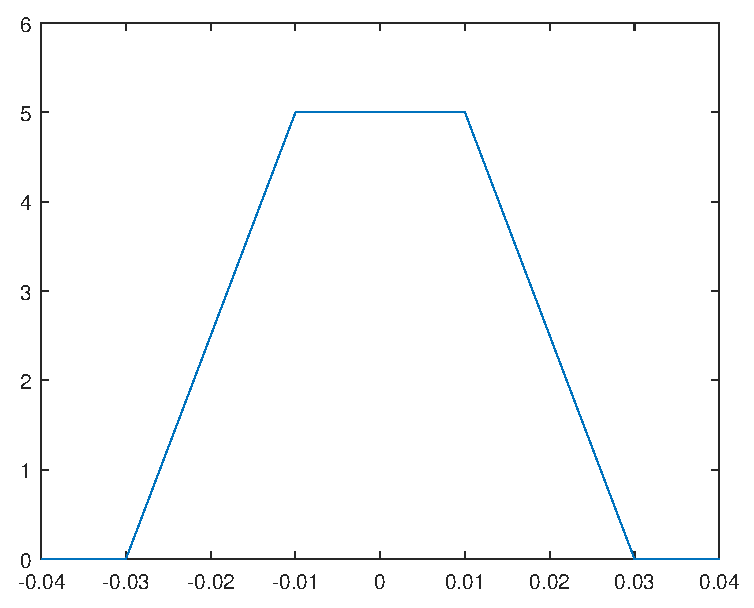
\includegraphics[scale=0.7]{lab1_06}
		\caption{Треугольный импульс} 
		\label{pic:lab1_06} % название для ссылок внутри кода
	\end{center}
\end{figure}
\subsubsection{Импульс с ограниченной полосой частот}
Сигнал имеет прямоугольный, то есть ограниченный по частоте спектр.
\begin{eqnarray}
y = \frac{\sin(\pi x)}{\pi x}
\end{eqnarray}
\begin{figure}[H]
	\begin{center}
		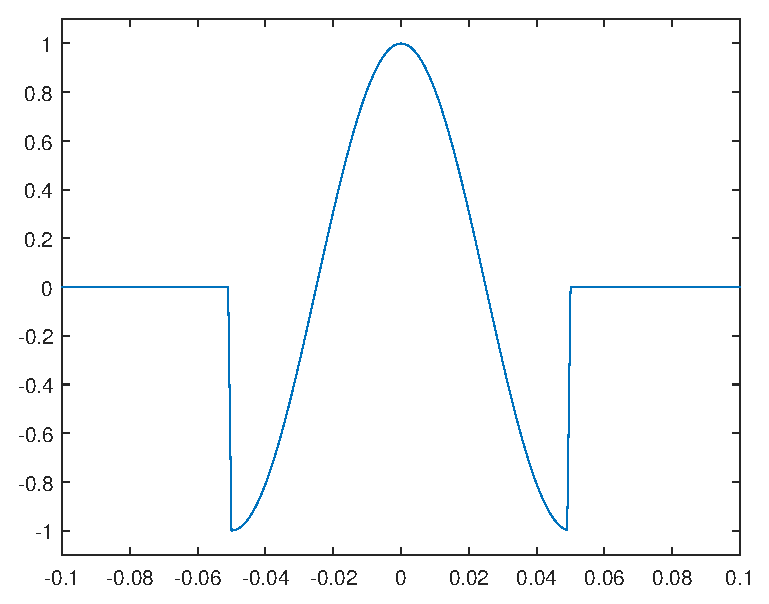
\includegraphics[scale=0.7]{lab1_07}
		\caption{Ограниченный по частоте импульс} 
		\label{pic:lab1_07} % название для ссылок внутри кода
	\end{center}
\end{figure}

\begin{figure}[H]
	\begin{center}
		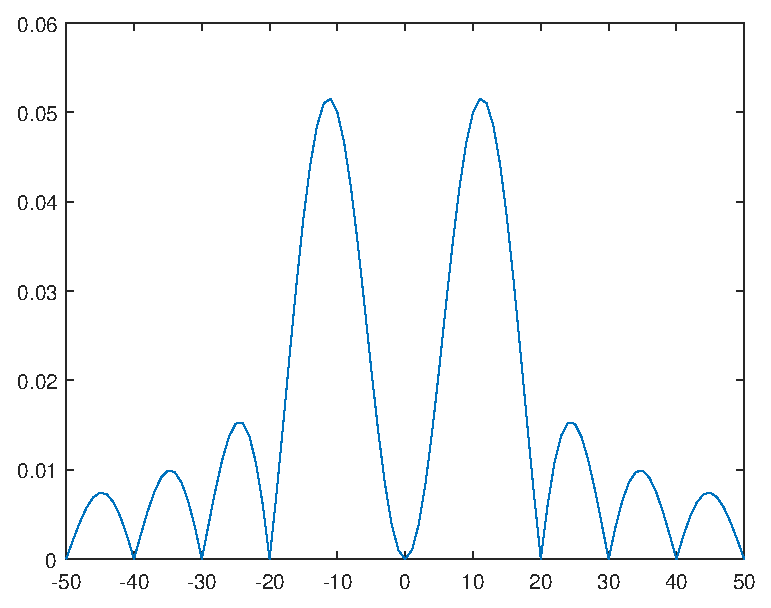
\includegraphics[scale=0.7]{lab1_08}
		\caption{Амплитудный спектр сигнала} 
		\label{pic:lab1_08} % название для ссылок внутри кода
	\end{center}
\end{figure}

\subsubsection{Импульс Гаусса}


\begin{eqnarray}
y = \exp(-\alpha t^2)\cos(2\pi f t)\\
\alpha = -\frac{5(2\pi f *bw)^2}{bwr *\log 10}
\end{eqnarray}

В этих формулах: t - значение времени, f - несущая частота, bw - относительная ширина спектра,
bwr - уровень в децибелах, покоторому производится измерение ширины спектра.

\begin{figure}[H]
	\begin{center}
		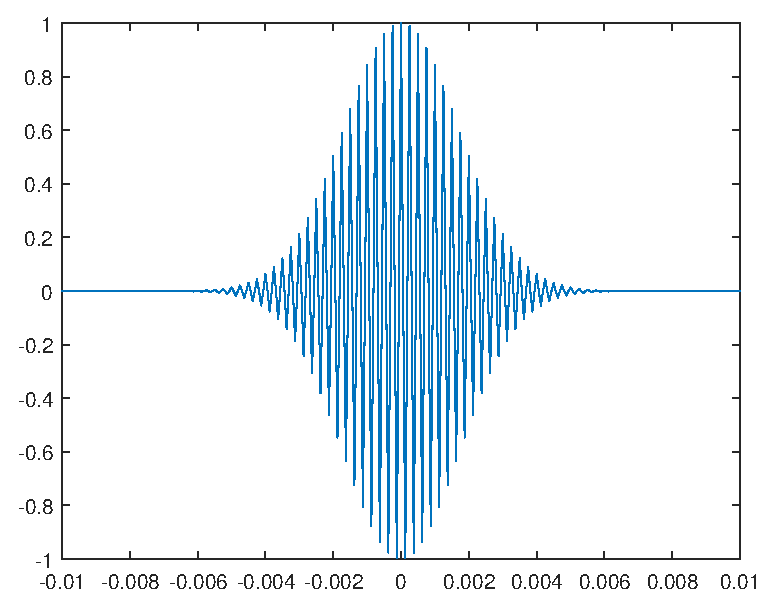
\includegraphics[scale=0.7]{lab1_09}
		\caption{Импульс Гаусса} 
		\label{pic:lab1_09} % название для ссылок внутри кода
	\end{center}
\end{figure}

\begin{figure}[H]
	\begin{center}
		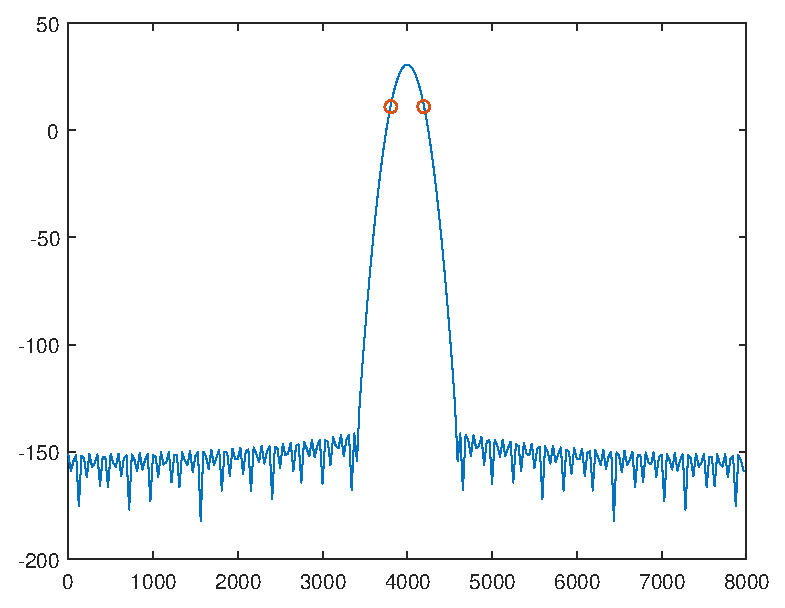
\includegraphics[scale=0.7]{lab1_10}
		\caption{Амплитудный спектр сигнала} 
		\label{pic:lab1_10} % название для ссылок внутри кода
	\end{center}
\end{figure}


\subsection{Генерация последовательности импульсов}

\begin{figure}[H]
	\begin{center}
		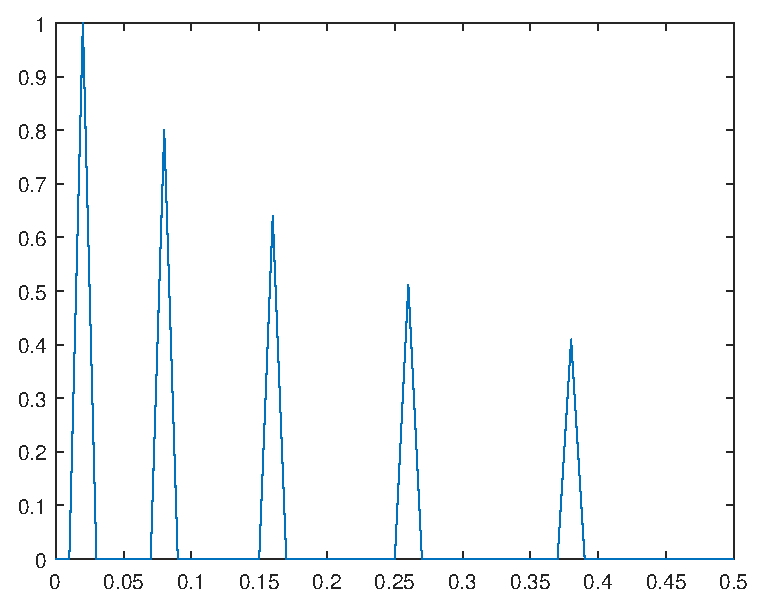
\includegraphics[scale=0.7]{lab1_11}
		\caption{Последовательность треугольных импульсов} 
		\label{pic:lab1_11} % название для ссылок внутри кода
	\end{center}
\end{figure}

\begin{figure}[H]
	\begin{center}
		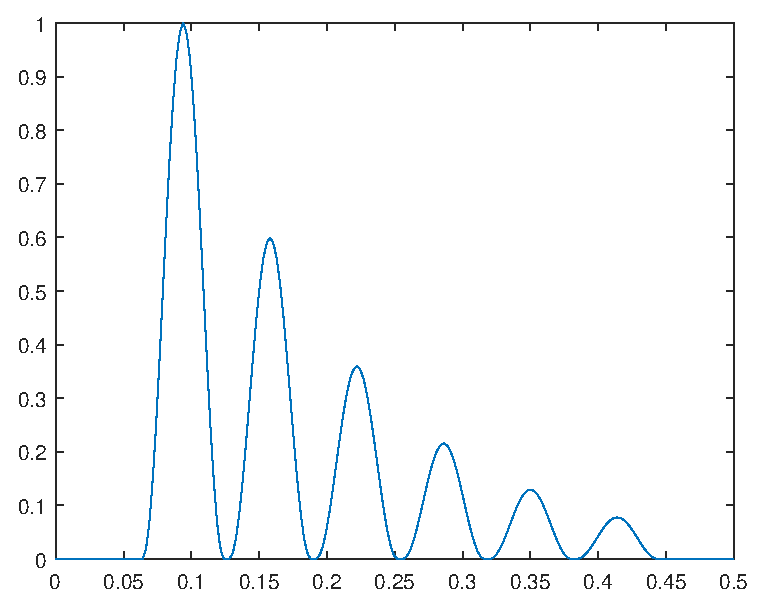
\includegraphics[scale=0.7]{lab1_12}
		\caption{Последовательность синусоидальных импульсов} 
		\label{pic:lab1_12} % название для ссылок внутри кода
	\end{center}
\end{figure}


\subsubsection{Последовательность прямоугольных импульсов}
\begin{figure}[H]
	\begin{center}
		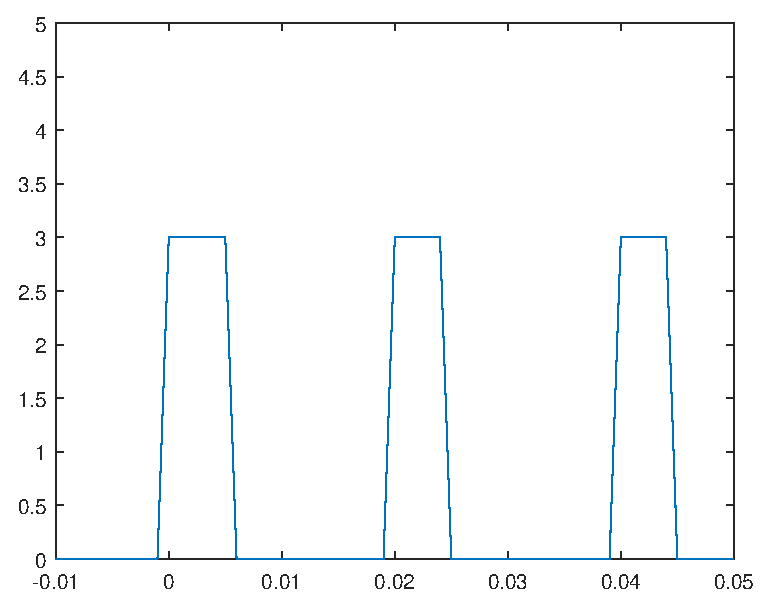
\includegraphics[scale=0.7]{lab1_13}
		\caption{Последовательность прямоугольных импульсов} 
		\label{pic:lab1_13} % название для ссылок внутри кода
	\end{center}
\end{figure}
\subsubsection{Последовательность треугольных импульсов}
\begin{figure}[H]
	\begin{center}
		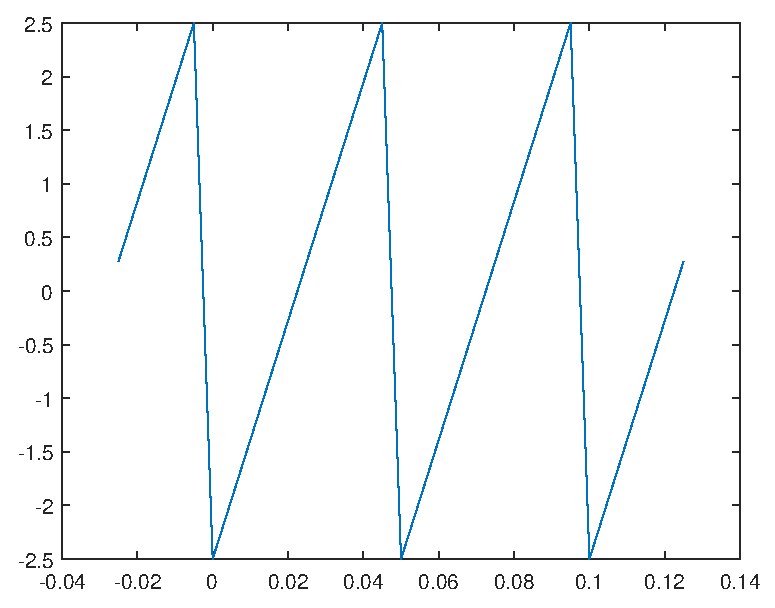
\includegraphics[scale=0.7]{lab1_14}
		\caption{Последовательность треугольных импульсов} 
		\label{pic:lab1_14} % название для ссылок внутри кода
	\end{center}
\end{figure}

\subsubsection{Функция Дирихле}

\begin{eqnarray}
diric(x) = \frac{\sin(n x/2)}{n \sin(x/2)}
\end{eqnarray}
В этой функции n - целое положительное число и определяет порядок.\\
Вид функции дирихле при нечётном порядке (n = 7)
\begin{figure}[H]
	\begin{center}
		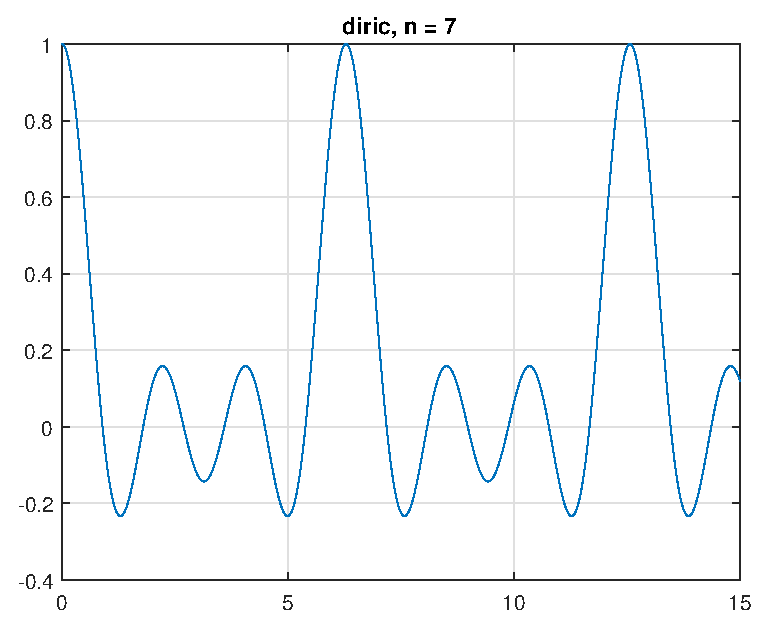
\includegraphics[scale=0.7]{lab1_15}
		\caption{Функция Дирихле при n = 7} 
		\label{pic:lab1_15} % название для ссылок внутри кода
	\end{center}
\end{figure}
Вид функции дирихле при чётном порядке (n = 8)
\begin{figure}[H]
	\begin{center}
		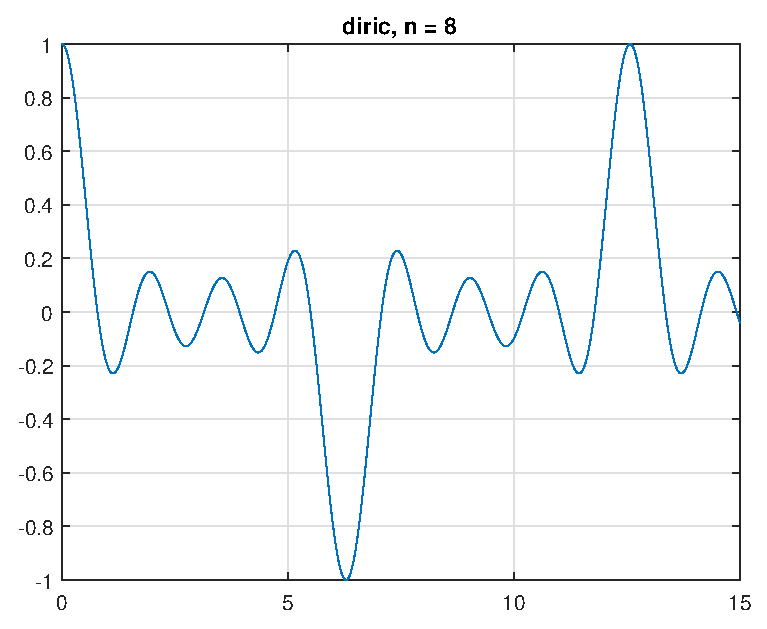
\includegraphics[scale=0.7]{lab1_16}
		\caption{Функция Дирихле при n = 8} 
		\label{pic:lab1_16} % название для ссылок внутри кода
	\end{center}
\end{figure}


\subsection{Сигнал с меняющейся частотой}
Сигналы разделяются по типу зависимости мнгновенной частоты от времени.
\subsubsection{Линейная зависимость}

\begin{eqnarray}
f(t) = f_0 + \beta t \\
\beta = \frac{f_1-f_0}{t_1}
\end{eqnarray}

\begin{figure}[H]
	\begin{center}
		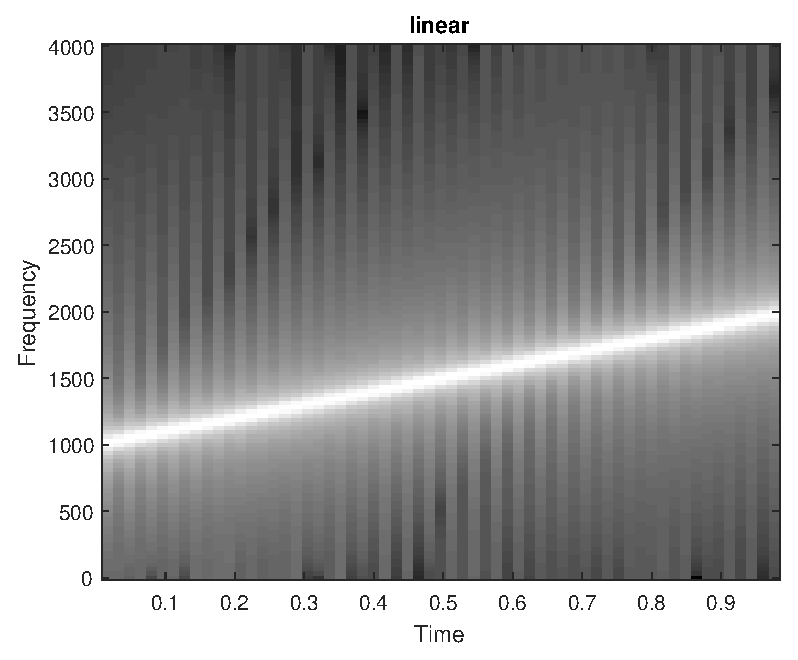
\includegraphics[scale=0.7]{lab1_17}
		\caption{Спектр сигнала при линейной зависимости} 
		\label{pic:lab1_17} % название для ссылок внутри кода
	\end{center}
\end{figure}


\subsubsection{Квадратичная зависимость}

\begin{eqnarray}
f(t) = f_0 + \beta t^2 \\
\beta = \frac{f_1-f_0}{t_1^2}
\end{eqnarray}

\begin{figure}[H]
	\begin{center}
		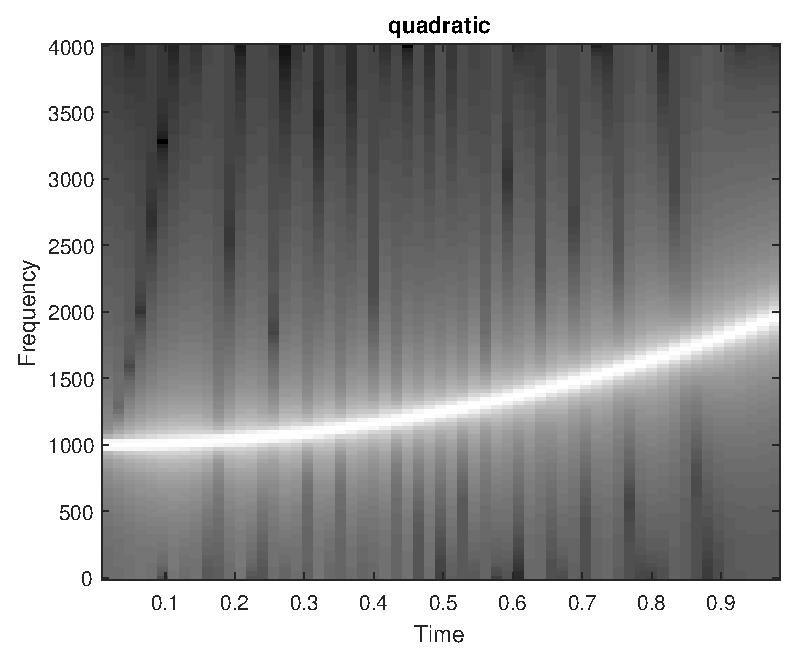
\includegraphics[scale=0.7]{lab1_18}
		\caption{Спектр сигнала при квадратичной зависимости} 
		\label{pic:lab1_18} % название для ссылок внутри кода
	\end{center}
\end{figure}


\subsubsection{Экспоненциальная зависимость}

\begin{eqnarray}
f(t) = f_0 + \exp(\beta t) \\
\beta = \frac{\ln(f_1-f_0)}{t_1}
\end{eqnarray}

\begin{figure}[H]
	\begin{center}
		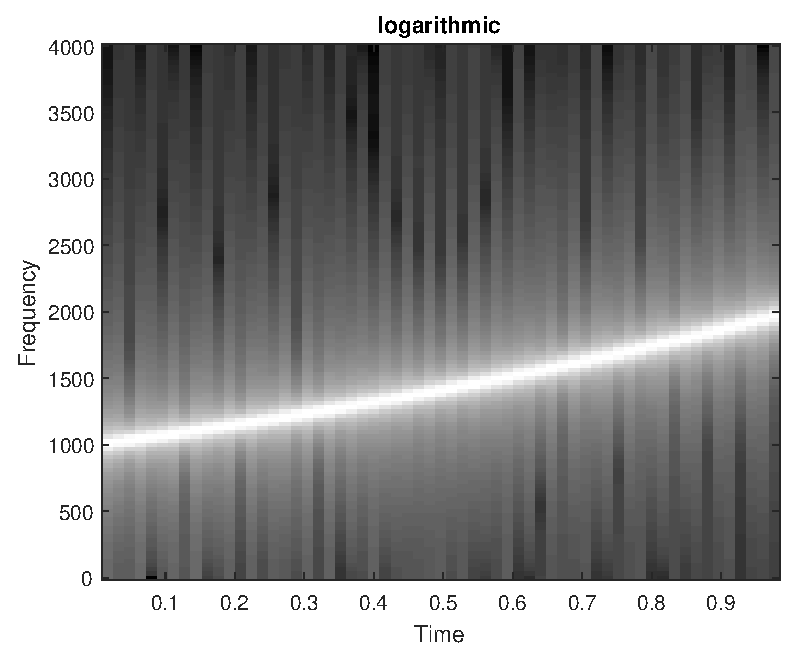
\includegraphics[scale=0.7]{lab1_19}
		\caption{Спект сигнала при экспоненциальной зависимости} 
		\label{pic:lab1_19} % название для ссылок внутри кода
	\end{center}
\end{figure}

\section{Вывод}
В ходе работы были рассмотрены различные способы визуализации сигналов,
способы получения спектра сигнала и методы генерации сигналов с разнообразными 
характеристиками. Так же были рассмотрены сигналы различного вида.


\newpage
\section{Приложение}
\subsection{Листинг}
% настрока частичного ввода (требуется один раз)
\makeatletter
\def\lst@PlaceNumber{\llap{\normalfont
                \lst@numberstyle{\the\lst@lineno}\kern\lst@numbersep}}
\makeatother

\lstinputlisting[
	label=code:code,
	caption={lab1.m},
]{lab1.m}
\parindent=1cm
\end{document}
